% =============================================================================
% Section à coller dans le rapport (fin / résultats expérimentaux)
% Dépendances utiles : \usepackage{graphicx,booktabs,siunitx,hyperref}
% Figure : docs/figures/cascade-v8-schema.png
% =============================================================================

\subsection*{Suspicion de fuite de données et nécessité d'une nouvelle cascade}

Lors des premières campagnes d'évaluation de l'ancienne cascade (DeBERTa~$\pm$~LLM), les scores obtenus (F1 en particulier) apparaissaient \textbf{anormalement élevés} au regard de la difficulté réelle de la tâche. Plusieurs indices convergent vers une \textbf{fuite de données} (\textit{data leakage}) non localisée avec certitude\,: chevauchement possible entre ensembles d'entraînement et de test, fuites liées aux pipelines d'évaluation antérieurs, ou contamination via des jeux dérivés. L'origine exacte n'a pas pu être isolée de façon définitive\,; en revanche, le diagnostic méthodologique est clair\,: \textbf{les métriques historiques ne sont pas fiables} tant que l'indépendance train/test n'est pas garantie.

Pour sortir de cette zone d'ambiguïté, l'équipe a évalué les modèles sur un \textbf{jeu jamais vu auparavant} par ces pipelines. Sur ce hold-out, l'accuracy observée est de l'ordre de \textbf{$\sim$80\,\%}\,: un résultat \emph{correct} mais \textbf{insuffisant} pour un déploiement d'annotation automatique exigeant. Ce constat a motivé la conception d'un \textbf{nouveau système en cascade V8}, plus transparent, plus contrôlé et évalué sur un gold standard humain indépendant.

\subsection*{Jeu d'évaluation gold (règle $\ge$\,3/6, batchs~1--3)}

Le gold utilisé pour l'évaluation de la cascade V8 est construit à partir des annotations humaines des batchs VLDBench~\textbf{1},~\textbf{2} et~\textbf{3}. Pour chaque paire, on ne retient un label de consensus que s'il existe un label clairement majoritaire avec au moins \textbf{3~accords} parmi jusqu'à~6 annotateurs (votes non \texttt{dismissed}). Les égalités en tête (ex.\ 3~supporting / 3~undetermined) sont \textbf{exclues} (aucun tie-break).

\begin{itemize}
    \item \textbf{2\,257} paires (cibles) retenues, réparties sur \textbf{413} références\,;
    \item distribution dominante\,: \texttt{not\_related} (1\,659), puis \texttt{undetermined} (518), \texttt{supporting} (79), \texttt{against} (1)\,;
    \item ce gold sert de référence pour mesurer l'accuracy et le F1 de la cascade V8 complète et de chaque étage.
\end{itemize}

\subsection*{Architecture de la cascade V8}

La cascade V8 orchestre trois étages de décision, puis calcule systématiquement le score de similarité\,:

\begin{enumerate}
    \item \textbf{Duo Zero Faute} (MiniLM~$0{,}4$ + DeBERTa Large~$0{,}6$)\,: auto-annotation seulement si les règles de confiance/accord sont satisfaites\,; sinon \emph{reject}.
    \item \textbf{Reranker undetermined} (détecteur binaire)\,: si $P(\texttt{undetermined})\ge 0{,}70$, label forcé \texttt{undetermined}\,; sinon passage à Qwen.
    \item \textbf{Qwen~7B} (prompt P3 + post-traitement métier)\,: dernier recours.
    \item \textbf{SBERT~v2}\,: cosine $\to$ champ \texttt{similarity\_annotation} (indépendant du choix de l'étage pour le label).
\end{enumerate}

\begin{figure}[htbp]
    \centering
    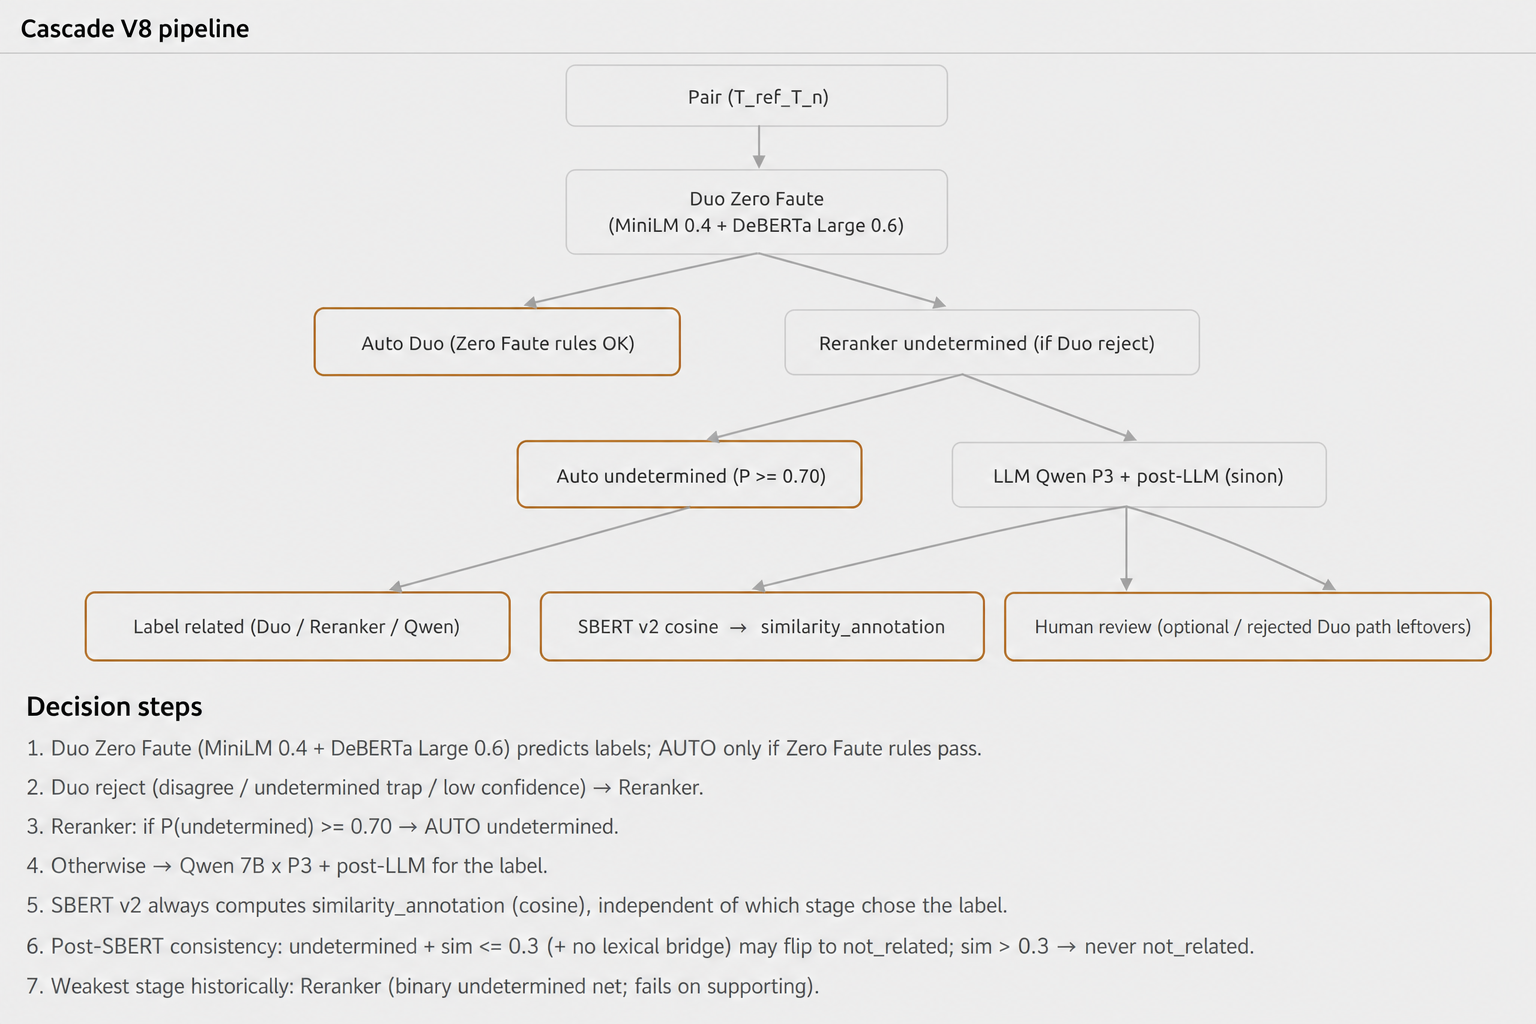
\includegraphics[width=0.92\textwidth]{figures/cascade-v8-schema.png}
    \caption{Cascade V8 pipeline (même convention visuelle que l'ancienne cascade DeBERTa$\to$Qwen)\,: Duo Zero Faute $\to$ Reranker undetermined $\to$ Qwen~P3, puis SBERT~v2 pour \texttt{similarity\_annotation}.}
    \label{fig:cascade-v8}
\end{figure}

\subsection*{Résultats globaux sur le gold $\ge$\,3/6}

Sur les 2\,257 paires, la cascade V8 obtient\,:

\begin{center}
\begin{tabular}{@{}lr@{}}
\toprule
Métrique & Valeur \\
\midrule
Accuracy & \textbf{94{,}2\,\%} \\
Erreurs & 131 / 2\,257 (5{,}8\,\%) \\
F1 weighted & 0{,}935 \\
F1 macro & 0{,}517 \\
Precision / Recall / F1 weighted & 0{,}936 / 0{,}942 / 0{,}935 \\
Precision / Recall / F1 macro & 0{,}583 / 0{,}508 / 0{,}517 \\
\bottomrule
\end{tabular}
\end{center}

Le F1 macro reste tiré vers le bas par la classe \texttt{supporting} (support faible, 79~cas) et \texttt{against} (1~cas)\,; le F1 weighted reflète mieux la masse \texttt{not\_related}.

\begin{center}
\begin{tabular}{@{}lrrrrr@{}}
\toprule
Classe (gold) & Support & Precision & Recall & F1 & Erreurs \\
\midrule
\texttt{not\_related} & 1\,659 & 0{,}985 & 0{,}990 & 0{,}988 & 16 \\
\texttt{undetermined} & 518 & 0{,}848 & 0{,}913 & 0{,}879 & 45 \\
\texttt{supporting} & 79 & 0{,}500 & 0{,}127 & 0{,}202 & 69 \\
\texttt{against} & 1 & 0{,}000 & 0{,}000 & 0{,}000 & 1 \\
\bottomrule
\end{tabular}
\end{center}

\subsection*{Performance par étage (Duo / Reranker / Qwen)}

Le routage des 2\,257 paires se répartit en Duo~1\,107 (49\,\%), Reranker~564 (25\,\%) et Qwen~586 (26\,\%).

\begin{center}
\begin{tabular}{@{}lrrrr@{}}
\toprule
Étage & $N$ & Accuracy & Erreurs & Taux d'erreur \\
\midrule
Duo Zero Faute & 1\,107 & \textbf{99{,}9\,\%} & 1 & 0{,}09\,\% \\
Qwen (fallback) & 586 & 93{,}0\,\% & 41 & 7{,}0\,\% \\
Reranker & 564 & \textbf{84{,}2\,\%} & 89 & 15{,}8\,\% \\
\bottomrule
\end{tabular}
\end{center}

Le \textbf{Reranker} est clairement le maillon le plus faible (\textit{le «\,cœur\,» fragile} de la cascade). Duo est quasi parfait sur les cas qu'il auto-annote (essentiellement des \texttt{not\_related} évidents). Qwen, en dernier recours, reste à 93\,\%.

\paragraph{Où le Reranker échoue.}
Ce n'est pas un classifieur 4~classes\,: c'est un \textbf{filet binaire \texttt{undetermined}}. S'il auto-annote, il ne peut prédire ni \texttt{supporting} ni \texttt{against}. Conséquence\,: dès qu'un vrai \texttt{supporting} arrive au Reranker, l'auto-annotation produit une erreur quasi certaine. Sur les 564 cibles Reranker\,:

\begin{itemize}
    \item \textbf{55} erreurs \texttt{supporting}$\to$\texttt{undetermined} (0/55 corrects sur le gold supporting)\,;
    \item \textbf{22} erreurs \texttt{undetermined}$\to$\texttt{not\_related} (souvent dues au post-traitement SBERT qui écrase un undet correct)\,;
    \item \textbf{11} erreurs \texttt{not\_related}$\to$\texttt{undetermined}\,;
    \item \textbf{1} erreur \texttt{against}$\to$\texttt{undetermined}.
\end{itemize}

Ces cas arrivent souvent au Reranker parce que le Duo, trop prudent, \emph{reject} au lieu d'auto-annoter (désaccord MiniLM/DeBERTa, piège undetermined, confiance basse).

\subsection*{Amélioration du Reranker}

Après diagnostic, une \textbf{version améliorée} du Reranker a été intégrée (en remplacement de l'ancien poids, chemin inchangé \texttt{reranker\_undetermined\_v8}). Évaluée sur les mêmes 564 cibles\,:

\begin{itemize}
    \item le nouveau modèle est \textbf{plus prudent}\,: davantage de \emph{reject} vers Qwen (133 vs $\sim$110)\,;
    \item sur les paires qu'il auto-annote encore, l'accuracy reste de l'ordre de \textbf{$\sim$83--84\,\%} (proche de l'ancien 84{,}2\,\% stocké cascade)\,;
    \item il \textbf{ne répare pas} à lui seul les 55 \texttt{supporting}$\to$\texttt{undetermined} lorsqu'il auto-annote (limite de design)\,;
    \item le gain attendu en cascade vient surtout du \textbf{renvoi vers Qwen} des cas limites, plutôt que d'un meilleur filet undetermined.
\end{itemize}

En perspective système\,: le passage d'une évaluation hold-out $\sim$80\,\% (ancienne cascade, jeu non contaminé) à \textbf{94{,}2\,\%} sur le gold $\ge$\,3/6 avec la cascade V8 montre le progrès global\,; le Reranker reste l'étage à renforcer (routage high-sim$\to$Qwen, seuil, post-SBERT, ou réentraînement avec négatifs durs \texttt{supporting}).

\subsection*{Erreurs par topic\,: volume vs structure}

Une analyse par topic montre que \textbf{Politics} concentre beaucoup d'erreurs en valeur absolue (107/131), mais cela reflète surtout son \textbf{poids dans le corpus} ($\sim$52\,\% des paires). Les taux d'erreur des autres topics restent généralement bas (souvent $<$4\,\%\,; Sports et Technology à 0\,\% sur ce gold). Autrement dit\,: les échecs ne s'expliquent pas principalement par un «\,sujet difficile\,» isolé\,; ils sont \textbf{structurels} (frontière \texttt{supporting}/\texttt{undetermined}, design du Reranker, post-SBERT), avec une répartition relativement homogène hors effet de volume Politics.

\subsection*{Synthèse}

\begin{enumerate}
    \item L'ancienne cascade a probablement \textbf{sur-estimé} ses performances (fuite suspectée)\,; un hold-out honnête donne $\sim$80\,\%.
    \item La cascade V8, évaluée sur un gold humain $\ge$\,3/6 (2\,257 paires, batchs~1--3), atteint \textbf{94{,}2\,\%} d'accuracy.
    \item Le Reranker est le goulot (84{,}2\,\%)\,: filet undetermined, faible sur \texttt{supporting}.
    \item Une version améliorée du Reranker a été déployée\,: plus prudente, utile surtout via le fallback Qwen.
    \item Les erreurs ne sont pas «\,un problème de topic\,» au sens fort\,: elles suivent surtout la mécanique du pipeline.
\end{enumerate}
